\section{Conclusion}
All in all, MongoDB is a powerful and popular documented-oriented database. It comes with a lot of features, which meets the modern-day requirements and challenges for business applications, platforms and the web. 
The examples about the MongoDB data model, queries and CRUD operations showed how easy it is for developers to setup and work with this database. MongoDB is also very flexible in terms of extending the structure of documents. However, it is strongly recommended to consider the usage of common patterns to create a strong and future-proof data model. The usage of patterns will also help developers to understand a given database structure and work together on larger projects.
Even in a big data context MongoDB is a good choice for big data applications. That is why you will find a lot of companies and startups using MongoDB in their development.

\subsection{MongoDB in CAP-Theorem}
In a single server or Master/Slave configuration MongoDB prioritize consistency over availability. That might be the reason why in most literature MongoDB is positioned at CP-side of the CAP-Theorem. But in \textit{Replica Sets} it is possible to trade some of the consistency for a higher availability, by configuring \textit{read preferences} (\ref{read-write}). By allow reading from secondaries, there is no way to ensure the client is reading consistent data. \anfuc{This behavior is characterized as eventual consistency, witch means that although the secondary's state is not consistent with the primary node state, it will become consistent over time}{p. 108}{Edward2015}. With \textit{write concerns} (\ref{read-write}) it is possible to obviate inconsistent reads happen to often, by ensure that a minimum number of secondaries is consistent. \\
Figure \ref{mongodb-cap} describes how the three values change depending on the configuration. The partition tolerance is always fulfilled, because MongoDBs architecture is designed that way. By allow reading from secondaries availability will be increased at the expense of consistency and some consistency can be recovered using \textit{write concerns}. But availability is always limited to reading, so it can never be fulfilled for all aspects of an application.
\begin{figure}[H]
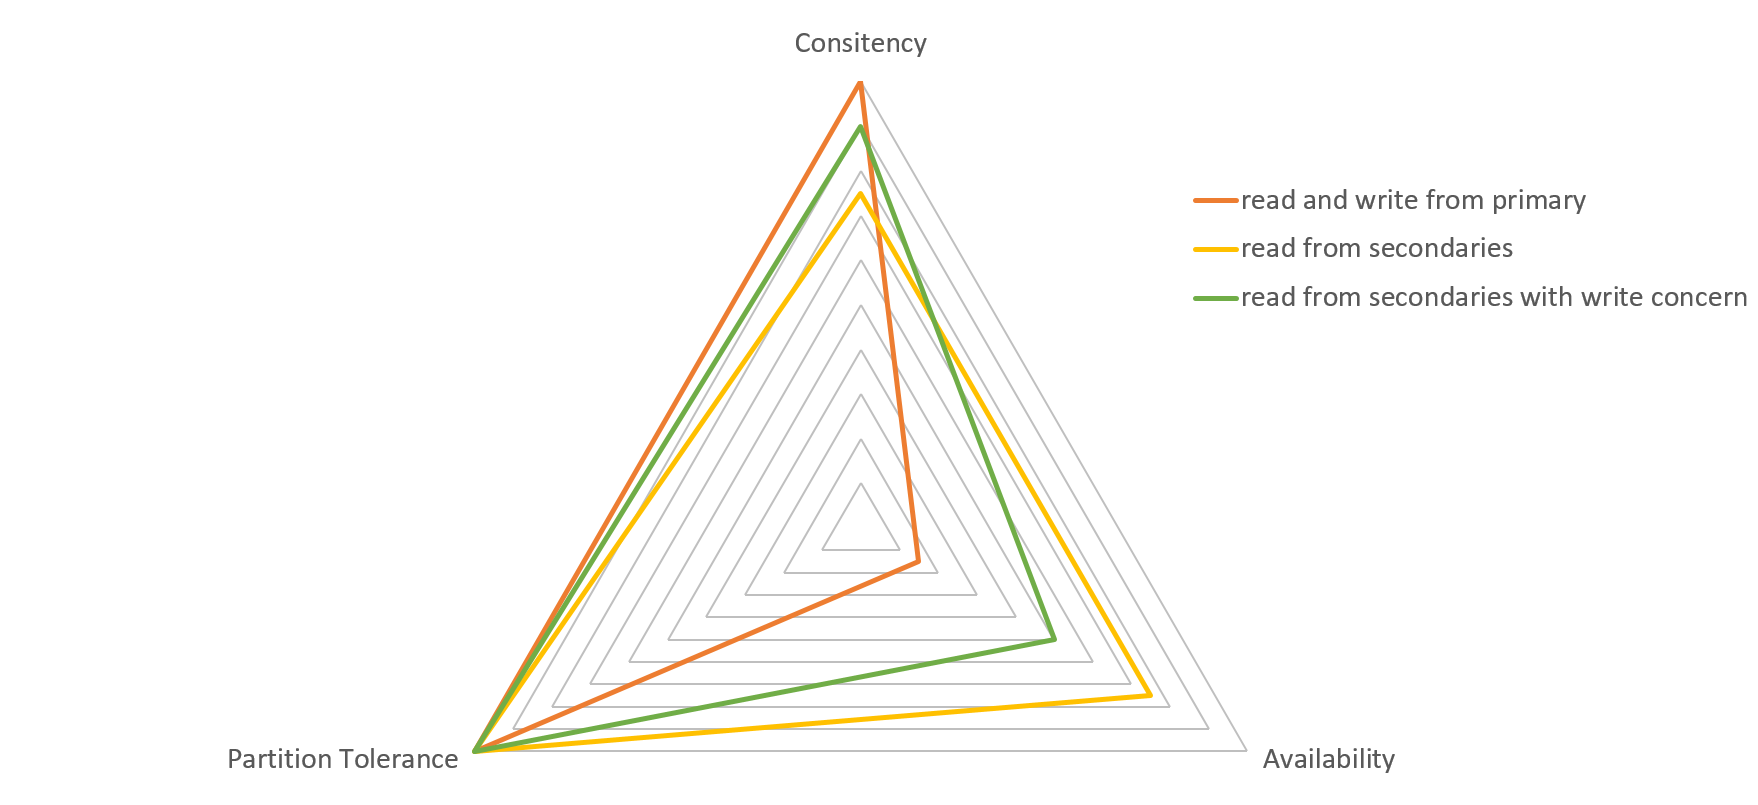
\includegraphics[width=\linewidth,keepaspectratio]{images/mongodb-cap.png}
\caption{Write process with write concerns}
\label{mongodb-cap}
\end{figure}